\documentclass{beamer}

\mode<presentation> 
{
    % The Beamer class comes with a number of default slide themes
    % which change the colors and layouts of slides. Below this is a list
    % of all the themes, uncomment each in turn to see what they look like.

    %\usetheme{default}
    %\usetheme{AnnArbor}
    %\usetheme{Antibes}
    %\usetheme{Bergen}
    %\usetheme{Berkeley}
    %\usetheme{Berlin}
    %\usetheme{Boadilla}
    %\usetheme{CambridgeUS}
    %\usetheme{Copenhagen}
    %\usetheme{Darmstadt}
    %\usetheme{Dresden}
    %\usetheme{Frankfurt}
    %\usetheme{Goettingen}
    %\usetheme{Hannover}
    %\usetheme{Ilmenau}
    %\usetheme{JuanLesPins}
    %\usetheme{Luebeck}
    \usetheme{Madrid}
    %\usetheme{Malmoe}
    %\usetheme{Marburg}
    %\usetheme{Montpellier}
    %\usetheme{PaloAlto}
    %\usetheme{Pittsburgh}
    %\usetheme{Rochester}
    %\usetheme{Singapore}
    %\usetheme{Szeged}
    %\usetheme{Warsaw}

    % As well as themes, the Beamer class has a number of color themes
    % for any slide theme. Uncomment each of these in turn to see how it
    % changes the colors of your current slide theme.

    %\usecolortheme{albatross}
    %\usecolortheme{beaver}
    %\usecolortheme{beetle}
    %\usecolortheme{crane}
    %\usecolortheme{dolphin}
    %\usecolortheme{dove}
    %\usecolortheme{fly}
    %\usecolortheme{lily}
    %\usecolortheme{orchid}
    %\usecolortheme{rose}
    %\usecolortheme{seagull}
    %\usecolortheme{seahorse}
    %\usecolortheme{whale}
    %\usecolortheme{wolverine}

%\setbeamertemplate{footline} % To remove the footer line in all slides uncomment this line
%\setbeamertemplate{footline}[page number] % To replace the footer line in all slides with a simple slide count uncomment this line

%\setbeamertemplate{navigation symbols}{} % To remove the navigation symbols from the bottom of all slides uncomment this line
}

\usepackage{graphicx} % Allows including images
\usepackage{booktabs} % Allows the use of \toprule, \midrule and \bottomrule in tables


\usepackage{beamerthemeshadow}
\usepackage{latexsym,amsbsy,amsopn,amstext,xcolor,multicol,amsmath}
\usepackage{amssymb,graphicx,wrapfig,fancybox}
\usepackage{pgf,pgfarrows,pgfnodes,pgfautomata,pgfheaps,pgfshade}
\usepackage{booktabs}
\usepackage{subfloat}
\usepackage{}
\graphicspath{{figures/}}

%----------------------------------------------------------------------------------------
%	TITLE PAGE
%----------------------------------------------------------------------------------------

\title[Work Report]{Measure of the Branching Ratio of the process\\ ${\eta}_c\rightarrow K^0_S K \pi$\\ via the decay $\psi(3686)\rightarrow \pi^0 h_c, h_c\rightarrow\gamma \eta_c$}

\author{Ma Hsuning}
\institute[NKU \& \& IHEP]
{
    Nankai Univ. \&\& IHEP\\
    \medskip
    \textit{maxn@ihep.ac.cn}
}
\date{\today}

%----------------------------------------------------------------------------------------
\begin{document}
%----------------------------------------------------------------------------------------
\frame{\titlepage}

%----------------------------------------------------------------------------------------
%----------------------------------------------------------------------------------------
\section{Over View}
\begin{frame}{}
\begin{block}{The purpose of our work}
Measure the branching ratio of the process ${\eta}_c\rightarrow K_S K \pi$, reducing the error measured before.\\
\bigskip
The process we study
\begin{center}
$\psi(3686) \rightarrow {\pi}^0 h_c, h_c \rightarrow \gamma {\eta}_c, {\eta}_c \rightarrow K^0_S K \pi$\\
${\pi}^0 \rightarrow \gamma \gamma, K^0_S \rightarrow {\pi}^+ {\pi}^-$
\end{center}
\end{block}
\end{frame}

%----------------------------------------------------------------------------------------
\begin{frame}{Method to do it}
\begin{block}{}
\begin{itemize}
\item Fit ${\eta}_c$ signal with invariant mass of $K_S^0$, $K$ and $\pi$(Corresponding to $N_{Obs1}$ and ${\epsilon}_1$);
\bigskip
\item Fit ${\eta}_c$ signal with the recoil mass of $\gamma$ and ${\pi}^0$(Corresponding to $N_{Obs2}$ and ${\epsilon}_2$);
\bigskip
\item The branching fraction will be acquired as the ratio of the two ${\eta}_c$ signal as
\end{itemize}
\begin{block}{}
\begin{center}
$Br({\eta}_c\rightarrow K_S^0 K \pi)=\frac{N_{Obs1}}{N_{Obs2}}\cdot \frac{{\epsilon}_2}{{\epsilon}_1} \cdot \frac{1}{Br(K_S^0 \rightarrow {\pi}^+ {\pi}^-)}$
\end{center}
\end{block}
\end{block}
\end{frame}

%----------------------------------------------------------------------------------------
\begin{frame}{Data Set}
\begin{itemize}
\item inclusive MC:     106M
\item signal MC:        200K for each of the inclusive process and exclusive process
\item BOSS version:     664p01
\end{itemize}
\end{frame}

%----------------------------------------------------------------------------------------
%----------------------------------------------------------------------------------------
\section{Exclusive Process}
\begin{frame}
\begin{block}{}
\begin{center}
\bigskip
\huge{the Exclusive Process}
\bigskip
\end{center}
\end{block}
\end{frame}
%----------------------------------------------------------------------------------------
\subsection{General Selection Criteria}
%----------------------------------------------------------------------------------------
\begin{frame}{Charged and Neutral Track Selection Criteria}
\begin{block}{Charged Tracks Selection Criteria}
\begin{itemize}
\item $ | \cos\theta |<0.93$
\item $|R_{z}|<10cm$,$R_{xy}<1cm$ (for the charged tracks NOT from $K^0_S$)\\ $2\le N_{good}\le 4$
\item No vertex cut for the charged tracks from $K^0_S$ \\ $N_{goodL}\ge 4$
\end{itemize}
\end{block}
\begin{block}{Neutral Tracks Selection Criteria}
\begin{itemize}
\item $E_{\gamma}>25 MeV$,$|\cos\theta|<0.8$ ( barrel region )
\item $E_{\gamma}>50 MeV$,$0.86<|\cos\theta|<0.92$ ( end-cap region )
\item $0\le t\le 14$ ( in unit of 50 ns)
\item $N_{\gamma}\le3$
\end{itemize}
\end{block}
\end{frame}
%----------------------------------------------------------------------------------------
\begin{frame}{$\pi^0$ List, $\gamma\pi^0$ List and Reconstruction of $K^0_S$}
\begin{block}{$\pi^0$ List and $\gamma \pi^0$ List}
\begin{description}
\item[$\pi^0$ list]
\begin{itemize}
\item $0.08<M_{\gamma\gamma}<0.2$ (With 1-C)
\item $N_{\pi^0}\ge 1$
\end{itemize}
\bigskip
\item[$\gamma\pi^0$ list]
\begin{itemize}
\item $2.8<M^{recoil}_{\gamma\pi^0}<3.2$
\item $3.3<M^{recoil}_{\pi^0}<3.7$
\end{itemize}
\end{description}
\end{block}
\begin{block}{Reconstruction of $K^0_S$}
\begin{itemize}
\item A primary vertex fit and a secondary vertex fit are performed
\item $ |M_{\pi \pi} - m_{K_S^0} | < 20 MeV/c^2$
\end{itemize}
\end{block}
\end{frame}
%----------------------------------------------------------------------------------------
\begin{frame}{Other Selection Criteria}
\begin{block}{Other Selection Criteria}
\begin{itemize}
\item Vertex Fit
\item 4-C Kinematic Fit
\item Minimum combined ${\chi}^2={\chi}_{4C}^2+{\chi}_{1C}^2+{\chi}_{pid}^2+{\chi}_{vertex}^2$ cut
\end{itemize}
\end{block}
\end{frame}
%----------------------------------------------------------------------------------------
\begin{frame}{Optimized Selection}
Using ROOT scripts, we got the Optimized Selection as below:
\begin{itemize}
\item $0<\chi_{4C}^2<25$;
\item $0.125<m_{\pi^0}<0.138$ (after 4-C);
\item $0.45<E(\gamma_{E1})<0.53$ (after 4-C);
\item $|m_{recoil}(\pi^0 \pi^0)-M_{J/\psi}|<0.033$;
\item $|m_{recoil}(\gamma)-M_{\chi_{c0}}|<0$;
\item $|m_{recoil}(\gamma)-M_{\chi_{c1}}|<0.004$;
\item $|m_{recoil}(\gamma)-M_{\chi_{c2}}|<0.002$;
\item $|m_{recoil}(\pi^+ \pi^-)-M_{J/\psi}|<0.004$. and exclusive process
\end{itemize}
\end{frame}
%----------------------------------------------------------------------------------------
\subsection{Preliminary Results}
\begin{frame}
\begin{columns}
\begin{column}{0.5\textwidth}
\begin{center}
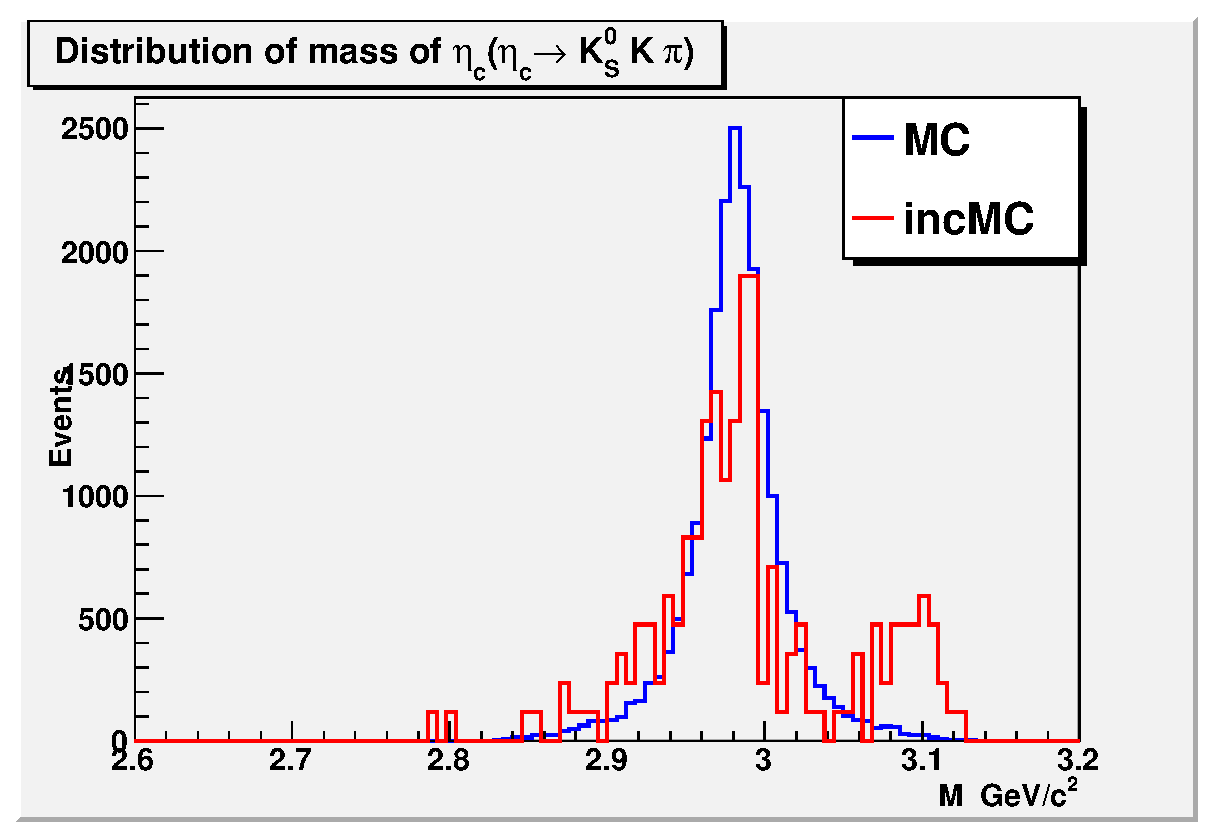
\includegraphics[width=1\textwidth,angle=0]{figures/Pi0hc_invariant_mass_of_etac.eps}\\
Mass distribution of $\eta_c$
\end{center}
\end{column}
\begin{column}{0.5\textwidth}
\begin{center}
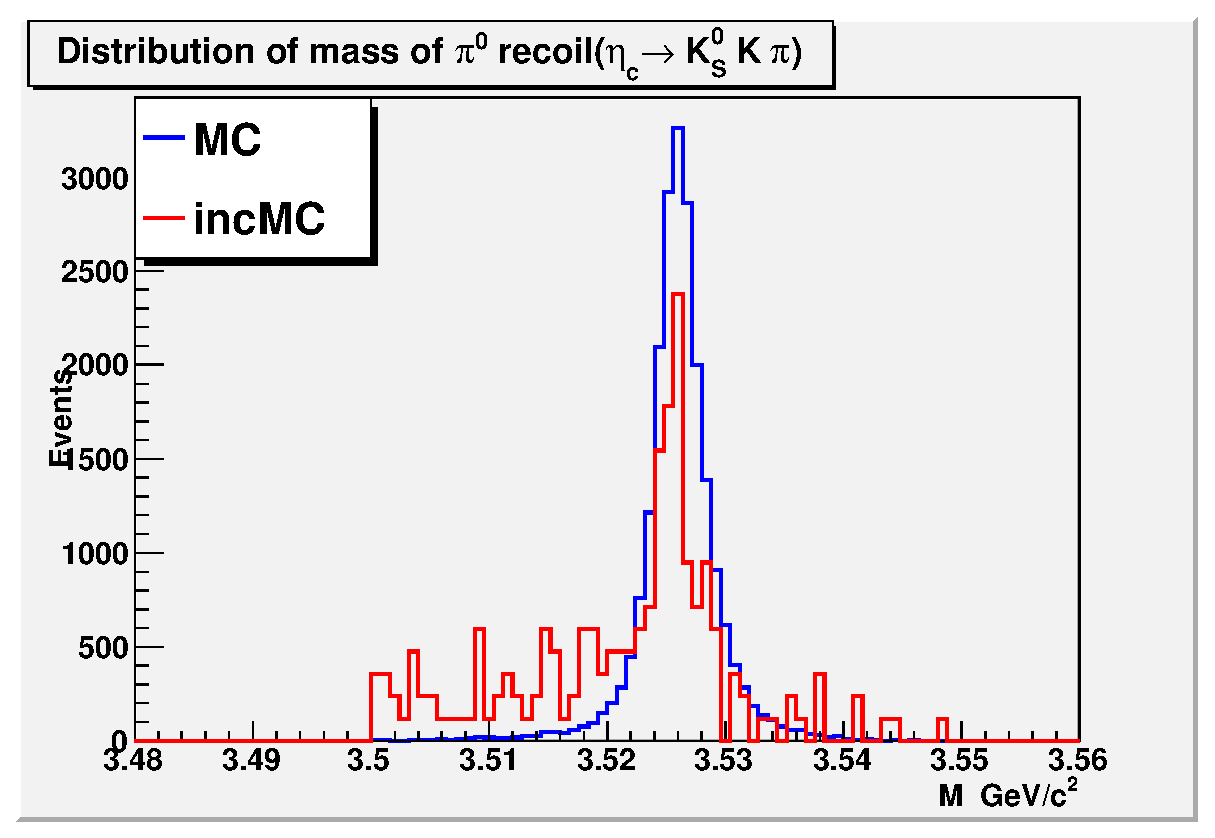
\includegraphics[width=1\textwidth,angle=0]{figures/Pi0hc_invariant_mass_of_hc.eps}\\
Mass distribution of $h_c$
\end{center}
\end{column}
\end{columns}
\end{frame}
%----------------------------------------------------------------------------------------
\begin{frame}{Topology analysis}
\vskip -1.5cm
\includegraphics[width=0.8\textwidth, angle=270]{figures/notice.eps}
\end{frame}

%----------------------------------------------------------------------------------------

%----------------------------------------------------------------------------------------
\section{Inclusive Process}
%----------------------------------------------------------------------------------------
\subsection{Event Selection}
\begin{frame}{Preliminary Event Selection}
\begin{block}{Selection of $\gamma_{E1}$ and $\pi^0$ candidates}
\begin{itemize}
\item $E_{\gamma}>25 MeV$,$|\cos\theta|<0.8$ ( barrel region )
\item $E_{\gamma}>50 MeV$,$0.86<|\cos\theta|<0.92$ ( end-cap region )
\item $465MeV < E({\gamma}_{{\rm E1}}) < 535MeV$
\item $120<M_{\gamma \gamma}<145 MeV/c^2$ ( With 1C )
\item photons used in $\gamma_{E1}$ candidates cannot form $\pi^0$ with another good photon
\item We keep the $\pi^0$ candidates with the minimum 1-C fit $\chi^2$ even if the daughter photons can be used in more than one $\pi^0$ candidates
\item We keep the events with only one $\pi^0$ in the $3.517-3.535GeV/c^2$ recoil-mass region.
\end{itemize}
\end{block}
\end{frame}
%----------------------------------------------------------------------------------------
\begin{frame}{Optimized Event Selection}
Using ROOT scripts, we got the Optimized Selection as below:
\begin{itemize}
\item $E(deposition)<0.6GeV$;
\item $|m_{recoil}(\pi^0 \pi^0)-M_{J/\psi}|<0.02$;
\item $|m_{recoil}(\gamma)-M_{\chi_{c0}}|<0.004$;
\item $|m_{recoil}(\gamma)-M_{\chi_{c1}}|<0.004$;
\item $|m_{recoil}(\gamma)-M_{\chi_{c2}}|<0.003$;
\item $|m_{recoil}(\pi^+ \pi^-)-M_{J/\psi}|<0.01$.
\end{itemize}
\end{frame}

%----------------------------------------------------------------------------------------
\subsection{Preliminary Results}
\begin{frame}
\begin{center}
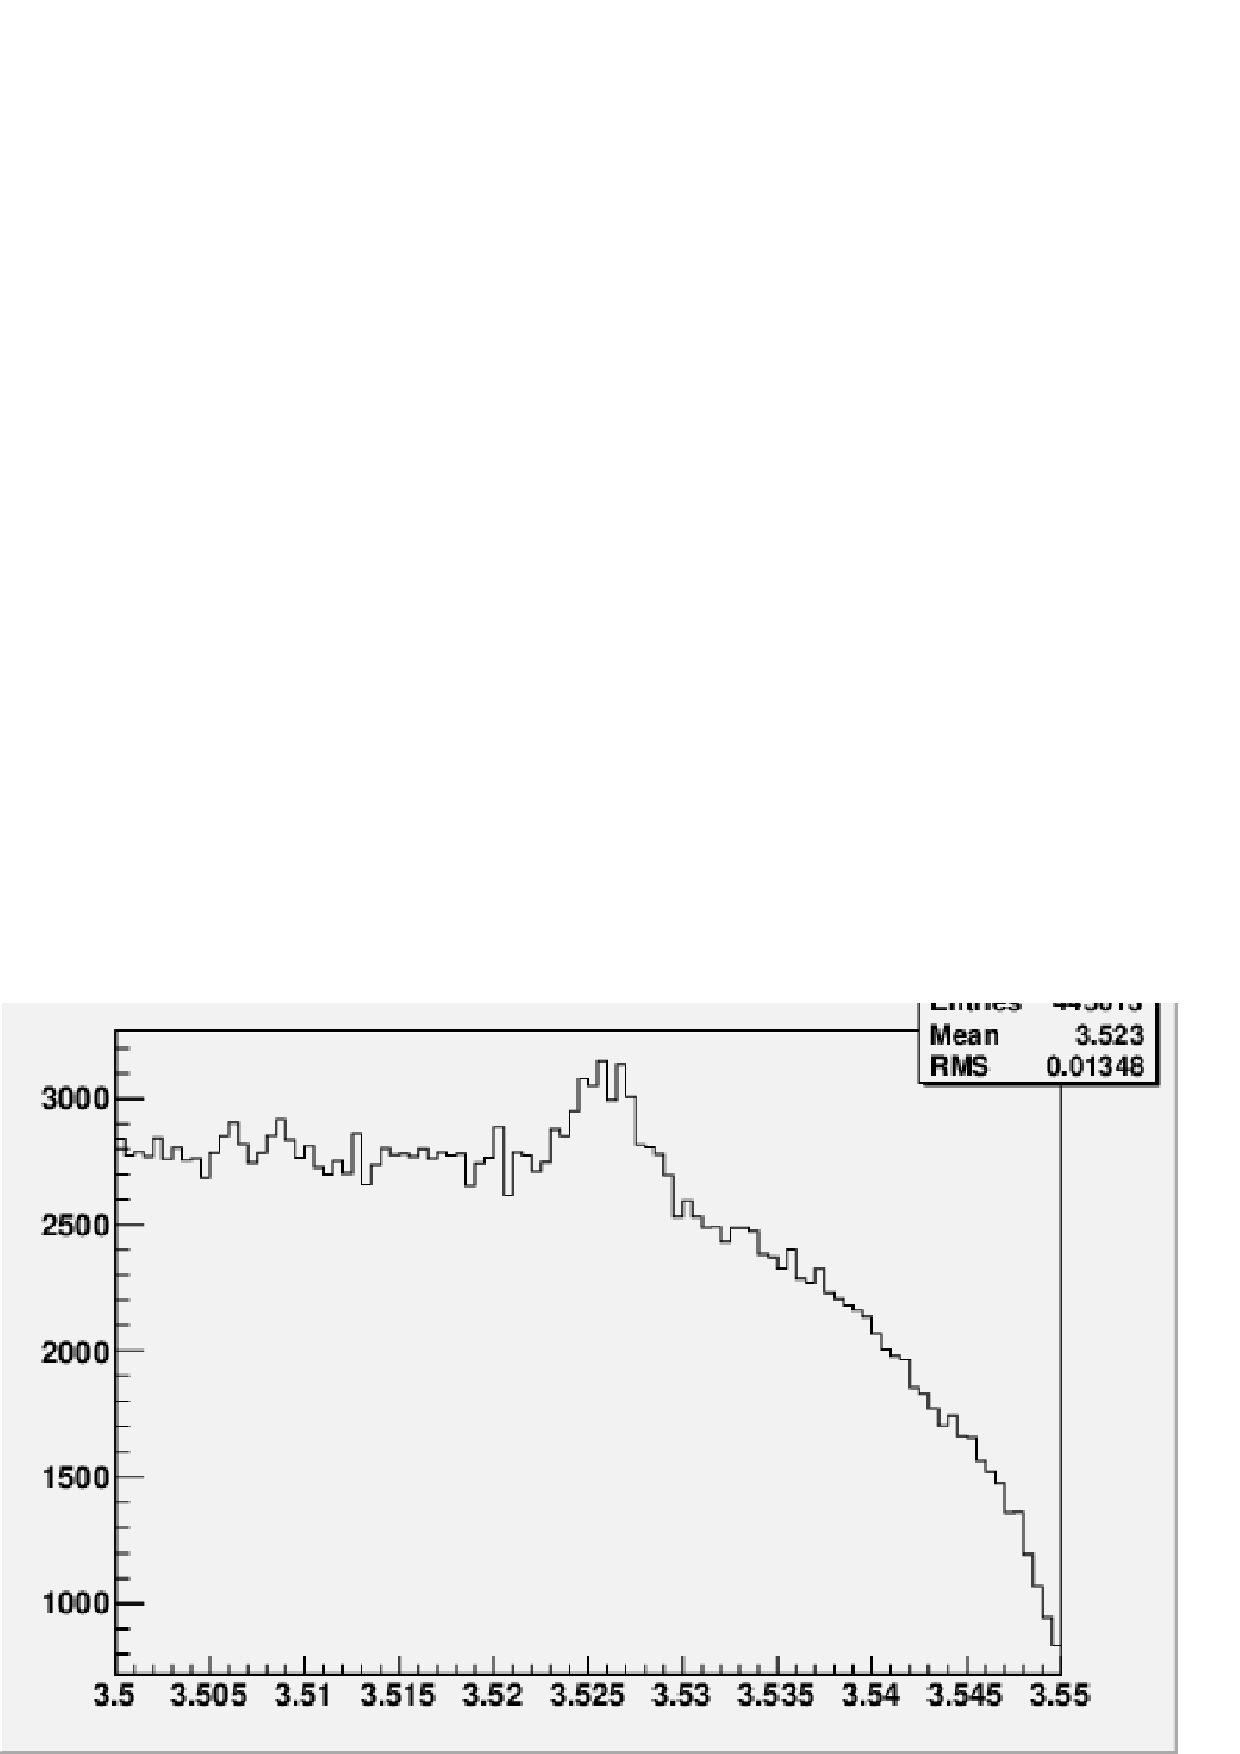
\includegraphics[width=0.8\textheight,angle=0]{figures/Pi0_recoil.pdf}\\
Mass distribution of $h_c$
\end{center}
\end{frame}
%----------------------------------------------------------------------------------------
\begin{frame}{Topology analysis}
\vskip -1.5cm
\includegraphics[width=0.8\textwidth, angle=270]{figures/notice_recoil.eps}
\end{frame}
%----------------------------------------------------------------------------------------

\section{Summery}
\subsection{Summery}
\subsection{Work to be done}
%----------------------------------------------------------------------------------------
\begin{frame}{}
%\begin{block}
\begin{itemize}
\item Fit the $\gamma$ $\pi^0$ recoil mass
\item Do IO check for inclusive process
\item Run data to get the branching ratio.
\end{itemize}
%\end{block}
\end{frame}

%----------------------------------------------------------------------------------------
\section{References}
\subsection{References}
\begin{frame}{References}
\begin{itemize}
\item  PRD \textbf{86}, 092009 (2012).
\item  PRL \textbf{104}, 132002 (2010).
\end{itemize}
\end{frame}
%----------------------------------------------------------------------------------------
\end{document}
